In order to devise a simple model for golf ball flight we first must understand some
prerequisite physics for projectiles and fluid dynamics for the airflow over the ball. Understanding
how the fluid flows over the surface of the ball is crucial to understanding the difference between
the flight of a golf ball and that of a standard projectile. Quantifying this effect will be a large
component of this project.

There has been significant work done previously in understanding the fluid dynamics around a golf ball
and how a golf ball flies. We will attempt to review some of this literature in this chapter and summarise
previous work on the topic.

First though, we must understand how normal projectiles fly without taking into account fluid dynamics effects.
\section{Projectile Motion}
A projectile is a body fired into the air by an initial impulse and then allowed to fall back to ground under the
action of gravity alone. This is the most naive and simplistic model of golf ball flight, completely
ignoring all aerodynamic effects, however we must understand it before building up to a more
complex model.

Consider motion in a 2 dimensional plane, labelled by $x$ along the horizontal and $y$ along the vertical.
A projectile is given an initial speed of the form $\vv_0 = (v_x, v_y)$. We set the origin of the coordinate system to be the point at the start of the
trajectory, $(x_0, y_0) = (0,0)$. In this problem the acceleration $(a_x,a_y)$ on the projectile, after the initial
impulse, is constant and of the form
\begin{equation} \label{grav}
a_x = 0, \quad a_y = -g
\end{equation}
where $g$ is the acceleration due to gravity. Since the acceleration is constant we can use
the standard formulas for motion under constant acceleration to derive the dynamics of the
projectile \citet{yandf}, which are
\begin{subequations} \label{suvat}
\begin{align}
v &= v_0 + at \label{v} \\
x &= v_0 t + \frac{1}{2} a t^2 \label{xsuvat} \\
v^2 &= v_0^2 + 2ax \\
x &= \left(\frac{v_0 + v}{2}\right) t .
\end{align}
\end{subequations}
Here $v = |\vv|$ is the speed at a time $t$, $x$ is the distance from the origin of the coordinate system,
$a$ is the component of the acceleration vector under consideration and $v_0 = |\vv_0|$ is the initial speed.

We will write the equations in component form along the axes. Let $\vv_0$ be the initial velocity.
In component form these will be
\[
v_{0x} = v_0 \cos \alpha
\]
along the $x$-axis and
\[
v_{0y} = v_0 \sin \alpha
\]
where $\alpha$ is the angle $\vv_0$ makes with the $x$-axis. Now using \eqref{grav}
and \eqref{v} we may find
\begin{subequations} \label{proj-v}
\begin{align}
v_x &= v_0 \cos \alpha \\
\shortintertext{and}
v_y &= v_0 \sin \alpha - gt . \label{proj-vy}
\end{align}
\end{subequations}

Now, using \eqref{xsuvat} (or by integrating \eqref{proj-v} with respect to $t$), we can obtain the 
standard formulas for the $x$ and $y$ positions during the flight of the projectile:
\begin{subequations}
\begin{align}
x &= (v_0 \cos \alpha) t \label{proj-x} \\
\shortintertext{and}
y &= (v_0 \sin \alpha) t - \frac{1}{2} g t^2 \label{proj-y} .
\end{align}
\end{subequations}

Eliminating $t$ between these equations demonstrates that projectiles follow parabolic
paths, giving
\begin{equation}
y = x \tan \alpha - \frac{g}{2v_0^2 \cos^2 \alpha} x^2
\end{equation}
for the path of the projectile.

Finally we may use these equations to find the maximum height, range and time of flight for a
projectile. The maximum height is obtained when $v_y = 0$ and solving \eqref{proj-vy} with this
condition gives
\begin{equation} \label{proj-height}
t_{H} = \frac{v_0 \sin \alpha}{g} .
\end{equation}
The range is obtained by solving for $y=0$ in \eqref{proj-y} and selecting the non trivial root for $t$
of
\begin{equation}
t_{F} = \frac{2 v_0 \sin \alpha}{g}
\end{equation}
where $t_{F}$ is the time of flight for the projectile. Inserting this into \eqref{proj-x} gives
\[
x = \frac{2 v_0^2 \cos \alpha \sin \alpha}{g}
\]
and recalling that $\sin 2 \alpha = 2 \cos \alpha \sin \alpha$ gives
\begin{equation}
x = \frac{v_0^2 \sin 2 \alpha}{g}
\end{equation}
for the range of the projectile.
\subsection{3D Projectile Motion}

Projectile motion in 3 dimensions works in exactly the same fashion as 2D projectile motion. Here we
will take the $z$-axis to be the vertical and $x$ and $y$ axes to be labelling the surface. After 
relabelling the coordinates in this fashion the only
component of acceleration is along the $z$-axis, with
\[
a_z = -g
\]
as before. All other equations remain the same.

\section{Basic Aerodynamics}

Of course, the flight of a golf ball is inevitably affected by aerodynamics. As such we need to have
some understanding of how aerodynamic effects will manifest themselves during the flight of the ball. 
In particular, we will need to understand how boundary layers
form on and separate from the surface of the golf ball and how this effects the lift and drag on the ball.
First we will review some basic fluid mechanics.

\subsection{Fluid Mechanics}

In this project we will model the air flowing around the ball as being an incompressible fluid. We will
consider an Eulerian description of fluid flow, viewing the motion as though the ball is fixed in the centre
of the coordinate system and the fluid moving around the ball \citet{Ruban2014}.

We will not concern ourselves with a full discussion of fluid mechanics from basic principles here, 
instead we will simply state some useful results predominantly following \citet{Ruban2014} and 
\citet{sears}.

Let $\vv$ be the fluid velocity, which is a function of the the position $\rvec$ from the origin of the
coordinate system and of time $t$. Let $\rho$ be the density of the fluid and $p$ the pressure. 
We define the material derivative to be (as a differential operator)
\begin{equation} \nonumber
\frac{D}{Dt} = \frac{\partial}{\partial t} + (\vv \cdot \nabla) .
\end{equation}
This derivative represents the rate of change of some quantity within the fluid, while moving with a small element
of the fluid flow. That is, in a description where the fluid moves relative to the coordinate system
the material derivative measures the rate of change as seen by a moving fluid element.

At all points within the fluid the mass continuity equation must apply
\begin{equation} \label{mass-cont}
\matdef{\rho} + \rho \nabla \cdot \vv = 0 .
\end{equation}
This equation encodes the condition that mass is conserved within a fluid without any sources or sinks.
In an incompressible fluid, as we will be primarily conserved with in this project, $\rho$ will not
change with time, and as such $D \rho / D t = 0$. As a consequence, both terms on the left hand side of
\eqref{mass-cont} must be zero everywhere within the fluid, and therefore the equation reduces to
\begin{equation} \label{incompress}
\nabla \cdot \vv = 0
\end{equation}
for an incompressible fluid.

The continuity equation gives one equation for the velocity components $u,v,w$\footnote{
	The convention within fluid mechanics is that the $x,y,z$ velocity components are called $u,v,w$
	respectively. That is \[
		v_x = u, \qquad v_y = v, \qquad v_z = w .
	\]
} within a fluid. In order to specify the pressure and velocity everywhere we therefore require three
more equations to determine the system. These three equations are supplied by considerations of
energy and momentum conservation. Keeping all of these in mind, we may write a
momentum equation in the form
\begin{equation} \label{momentum}
\rho \matdef{\vv} = - \nabla p + \mu \nabla^2 \vv + \ff
\end{equation}
where $\ff$ is body force per unit volume acting on the fluid (for example a gravitational force) 
and $\mu$ is the viscosity of the fluid.

Equations \eqref{incompress} and \eqref{momentum} when taken together form the Navier-Stokes equations
for the velocity and pressure fields within an incompressible fluid. It is well known that these
equations are highly non-linear and exceedingly difficult to solve both analytically and numerically,
except in special circumstances.

From solutions of the Navier-Stokes equations emerges a number of fascinating effects within fluid 
dynamics. In this project, we are particularly interested in boundary layer effects and turbulence.

\subsection{Non Dimensional Variables and the Reynolds Number}

In physics we are often interested in understanding the behaviour of a system independent of a
choice of units \citet{0143-0807-31-4-019}. Instead, we wish to
have a system of measurement which does not depend intrinsically on one set on units, but on more 
fundamental ideas such as length or mass. We desire this for two main reasons:
\begin{itemize}
	\item Physical statements should not have any dependency on the units they are stated in.
	Non-dimensionalising the problem ensures that this is the case.
	\item Using non-dimensional variables allows problems of different scales to be compared to each 
	other on an equal footing. Often the points when the physical behaviour of the system changes 
	will depend on some non-dimensional parameter, as we will see with turbulence later.
\end{itemize}

Additionally, analysing the fundamental dimensions of a physical problem can yield information on the
functional form of quantities within the model without having to use more advanced mathematical
techniques to derive such results. By simply understanding the dependency on fundamental units we
often can find interesting scaling laws for functions of interest.

The fundamental dimensions (only those which will be useful in this project) are as follows:
\begin{table}[h]
\centering
\begin{tabular}{l c}
Dimension & Symbol \\
\hline
Length & $L$ \\
Mass & $M$ \\
Time & $T$
\end{tabular}
\caption[List of fundamental dimensions]{List of fundamental dimensions we will require in this report.}
\end{table}

Any quantities of interest can be written using these variables: for example, an area $A$ would have 
the dimensions $[A] = L^2$ and a velocity $[V] = L/T$.

Physical laws can, in general, be written as, \citet{0143-0807-31-4-019}
\begin{equation} \label{functional}
q_{0} = f(q_1,q_2,\ldots,q_n)
\end{equation}
where $q_0$ is a physical quantity we are interested in obtaining, $q_1,\ldots,q_n$ are independent
physical quantities and $f$ is a functional relationship between them.

When analysing the dimensions of a problem we must ensure that the following conditions are
satisfied
\begin{itemize}
\item Both sides of \eqref{functional} must have the same fundamental dimensions.
\item Any sum of $q_i$ must have the same dimensions.
\item Any function of $q_i$ (say, exponential or trigonometric) must be dimensionless. This is as a 
direct result of the last condition and being able to expand these functions as a power series.
\end{itemize}

We will demonstrate this technique in section~\ref{sec:drag}.

One of the aims of dimensional analysis is to find groupings of physical quantities which are
dimensionless. These have useful properties of scale invariance which leads to natural parameterisations
for physical problems. A key result in finding such dimensionless groupings is the Buckingham $\pi$ 
theorem, which states the following:

\begin{bucktheorem}[Buckingham $\pi$]
Consider a physical law in the form of \eqref{functional}. Let there be $n$ parameters $q_1,q_2,\ldots,q_n$,
and $k$ fundamental units in which these parameters may be written. Then there exist $n-k$ dimensionless
parameters $\pi_i$ which satisfy
\[
F(\pi_1, \ldots, \pi_{n-k}) = 0
\]
for some function $F$ \citet{0143-0807-31-4-019}.
\end{bucktheorem}

Within fluid mechanics one such dimensionless grouping which manifests often is the Reynolds
number, defined as 
\begin{equation} \label{re-number}
Re = \frac{\rho v L}{\mu} .
\end{equation}
For a sphere, $v, \mu$ and $\rho$ are defined as they have already been in this text, and the
characteristic length $L$ is defined to be the diameter of the sphere.
The Reynolds number represents the ratio of inertial forces to viscous ones, and we will make considerable
use of it within the project. The Reynolds number, in some ways, can be considered to be a non
dimensional analogue of the velocity, taking into account the intrinsic length scale of the problem
under consideration.

\subsection{Boundary Layers}

One of the fundamental ideas within fluid mechanics is that of the no slip condition. The no slip 
condition specifies that when a fluid encounters a solid body it must, at the surface of the body,
take the velocity and temperature of that body. 

The concept of the boundary layer was introduced by Ludwig Prandtl in 1904 at the International
Mathematics Congress. Initially the utility of the ideas Prandtl presented were not appreciated, however
Prandtl's ideas have shaped fluid mechanics in the century after his work was presented.

For high Reynolds numbers the flow can be divided into two portions: the free stream flow where the
fluid moves quickly and viscous effects are unimportant, and a thin layer of fluid around the body 
called the boundary layer where viscous effects come into play. The origin of this thin layer of fluid
is the no slip condition: at the surface of the body the fluid must take the velocity of the body itself.
However, as we move away from the body the fluid very quickly returns to the free stream velocity. The
domain over which this rapid change in velocity occurs is the boundary layer.

The equations which govern the flow within the boundary layer are a simplified version of the
Navier-Stokes equations, taking into account the order of magnitude of the boundary layer compared to
the size of the body. The derivation of these equations is completed by scaling the Navier-Stokes 
based on the assumption that the boundary layer is much smaller than the body size \citet{anderson}.

Boundary layer theory has been hugely important in the development of aerodynamics, taking previously
intractable problems and facilitating a better understanding of the fluid dynamics over bodies 
\citet{anderson}. The affect of the boundary layer will be important in the modelling of golf balls,
as we will see later.

\subsection{Lift and Drag} \label{sec:drag}

In order to go beyond modelling golf ball flight as simply that of a projectile we must understand 
how the lift and drag forces affect the flight of the ball. We can use dimensional analysis arguments
to obtain a functional form for these effects. Here we follow the analysis of 
\citet{0143-0807-31-4-019} and \citet{anderson} in order to demonstrate the analysis for the drag force. 
The lift is found in a similar way.

One first must ask what physical terms we would expect the drag to have a dependency on. We would
expect some dependency on the velocity $v$ of the object through the fluid, on the shape of the body and
a characteristic length scale $r$ for the body, on the density of the fluid $\rho$, and finally on
the viscosity of the fluid $\nu$.

Forming an equation in the style of \eqref{functional} between these quantities and the drag force 
$D$ we obtain
\begin{equation} \label{drag-dimensions}
D = k f(v, r, \rho, \nu)
\end{equation}
where $k$ is a dimensionless constant which will take into account the shape of the body and
potentially other dimensionless parameters such as the Reynolds number \eqref{re-number}.

We attempt to obtain values of $\alpha, \beta, \gamma, \delta$ which balances \eqref{drag-dimensions}.
The dimensions of the quantities in \eqref{drag-dimensions} are as follows:
\begin{equation} \nonumber
[D] = M L T^{-2}, \qquad [v] = L T^{-1}, \qquad [r] = L, \qquad [\rho] = M L^{-3}, \qquad [\nu] = M L^{-1} T^{-1}
\end{equation}
and so balancing \eqref{drag-dimensions} implies that
\begin{equation}
M L T^{-2} = M^{\gamma + \delta} L^{\alpha + \beta - 3\gamma - \delta} T^{-\alpha-\delta} .
\end{equation}

Equating the powers leads to a system of 3 linear equations in 4 variables for each fundamental unit
given by
\begin{subequations}
\begin{align}
1 &= \gamma + \delta \\
1 &= \alpha + \beta - 3 \gamma - \delta \\
-2 &= \alpha - \delta
\end{align}
\end{subequations}
for $M, L$ and $T$ respectively.

Using these equations we can eliminate all but one of the parameters, and by application of the Buckingham
$\pi$ theorem we expect that there will be $4-3=1$ dimensionless parameters. Writing all these in terms
of $\delta$ we can find
\begin{align}
D &= k v^{2-\delta} r^{2-\delta} \rho^{1-\delta} \nu^{\delta} \\
\shortintertext{and rearranging these powers}
D &= k \rho r^2 v^2 \left(\frac{\nu}{\rho r v}\right)^{\delta} .
\end{align}
We can then recognise that the term in the brackets is $1/Re$. Since the Reynolds number is raised to
an arbitrary power $\delta$ we can include the constant $k$ and the $Re^{-\delta}$ into one functional
form, $f(Re)$, which accounts for the dimensionless factor. Writing into this form gives
\begin{equation} \label{drag-functional}
D = f(Re) \rho r^2 v^2 .
\end{equation}
Notice that now we have $[D] = [\rho r^2 v^2] = MLT^{-2}$ as we expect. 
The form of $f$ depends on the velocity of the body moving through the fluid.

There are two separate cases of drag which occur in nature. The low Reynolds number case and the
high Reynolds number case. In this project we will be concerned with the high Reynolds number case,
where drag takes the form of \eqref{drag-functional}. However, in the low Reynolds number case the form
of the drag is \citet{0143-0807-31-4-019}
\begin{equation}
D = k \nu r v
\end{equation}
which is known as Stokes drag. We will not consider this form in this project.

Within the literature related to fluid dynamics and aerodynamics \eqref{drag-functional} is normally written
with different names for the variables, namely 
\begin{equation} \label{drag}
F_{D} = \frac{1}{2} \rho \vv^2 A c_{D}
\end{equation}
where $F_{D}$ is the drag force, and $c_{D}$ is the dimensionless drag coefficient which depends on 
the Reynolds number. It is this form
we will use from here on. 

An expression for the lift can be derived using very similar analysis, and has the same form as the
drag:
\begin{equation} \label{lift}
F_{L} = \frac{1}{2} \rho \vv^2 A c_{L}
\end{equation}
where here $c_{L}$ is the lift coefficient.

\subsection{Boundary Layer Separation}

Boundary layer separation is a phenomena whereby the boundary layer of an object ``peels'' away from
the body and forms a wake behind the body. The idea of boundary layer separation was also introduced
by Prandtl in 1904 at the same time as presenting his initial work on boundary layers.

The mechanism by which this occurs is the flow in the 
boundary layer moving against an adverse pressure gradient \citet{FLM:374505}. As the fluid in the boundary layer moves
against the adverse pressure gradient, the speed of the fluid slows until eventually coming to a
complete stop and then proceeding back in the direction it arrived. At this point the fluid moves away
from the body, expanding the boundary layer at the separation
point beyond the usual thickness of the layer.

The fluid which has detached from the body then begins to form vortices in the wake behind the body,
increasing the drag on the body considerably as the pressure at the front and back of the body changes
considerably.

\subsection{The Magnus Effect}

In addition to the drag forces which we have discussed in the previous section, there is another
major effect from the motion of the fluid on golf ball trajectories: the Magnus effect. The Magnus
effect is caused by the spin of the ball moving through the fluid medium, and accounts for large
deviations from a trajectory not considering the effect \citet{Seifert2012}.

In the Magnus effect, the boundary layer around the spinning body separates from the body at different
points and forms a wake behind the body which does not point in the direction of motion.
\begin{figure}[h]
\centering
\begin{subfigure}{.3\textwidth}
\begin{tikzpicture}
\draw (0,0) circle (1.4);
\node[label=Ball] at (0,-0.4) {};
\draw[-open triangle 45] (1,1.8) -- (1,1);
\draw[-open triangle 45] (-1,-1.8) -- (-1,-1);
\node[label=Lower separation point] (l) at (0,-2.4) {};
\node[label=Upper separation point] (u) at (0,1.5) {};
\draw[draw=red,-triangle 90] (0.3,-0.3) -- (1.4,-1.4);
\draw[draw=blue,-triangle 90] (-0.4,0) -- (-1.7, 0);
\node at (0,-1) (one) {};
\node at (-1,0) (two) {};
\draw[draw=green] (two) edge[out=270,in=180,->] (one);
\end{tikzpicture}
\caption{Boundary layer separation}
\end{subfigure}
\quad \qquad
\begin{subfigure}{.3\textwidth}
\begin{tikzpicture}
\draw (0,0) circle (1.4);
\node[label=Ball] at (0,-0.4) {};
\draw[-open triangle 45] (-1,1.8) -- (-1,1);
\draw[-open triangle 45] (1,-1.8) -- (1,-1);
\node[label=Lower separation point] (l) at (0,-2.4) {};
\node[label=Upper separation point] (u) at (0,1.5) {};
\draw[draw=red,-triangle 90] (0.3,0.3) -- (1.4,1.4);
\draw[draw=blue,-triangle 90] (-0.4,0) -- (-1.7, 0);
\node at (0,-1) (one) {};
\node at (-1,0) (two) {};
\draw[draw=green] (one) edge[out=180,in=270,->] (two);
\end{tikzpicture}
\caption{Reversed boundary layer separation}
\end{subfigure}
\caption[Diagram of the separation points in the Magnus Effect]{Here we see the two scenarios for
boundary layer detachment. The red arrow indicates the direction which the detached boundary layer
proceeds in, the blue the direction of the ball, and the green arrow the direction of spin of the
ball.}
\label{separation}
\end{figure}

The points at which the boundary layer separates from the body at the top and
bottom of the ball make a significant difference to the direction in which the wake will point: if
the boundary layer at the top of the ball separates later than the bottom (see Figure \ref{separation}a) 
then we will have a positive Magnus effect, and the lift will be increased. In the opposite case, 
where the bottom separates later than the top, we will have a negative Magnus effect 
(see Figure \ref{separation}b) and the lift on the ball will be decreased or potentially act to
push the ball further towards the ground.

The fluid behind the rotating sphere will become turbulent as the sphere leaves a gap which the wake
refills as it passes. This mechanism is important while modelling the golf ball later, as the size
of the turbulent wake will affect the drag on the ball.

In Figure \ref{magnus} we see a representation of the streamlines over a sphere. Here we have laminar
flow in the boundary layer. However this is not always the case, if the flow is turbulent within the boundary
layer before separation the drag can change considerably. 

\begin{figure}[h]
\centering
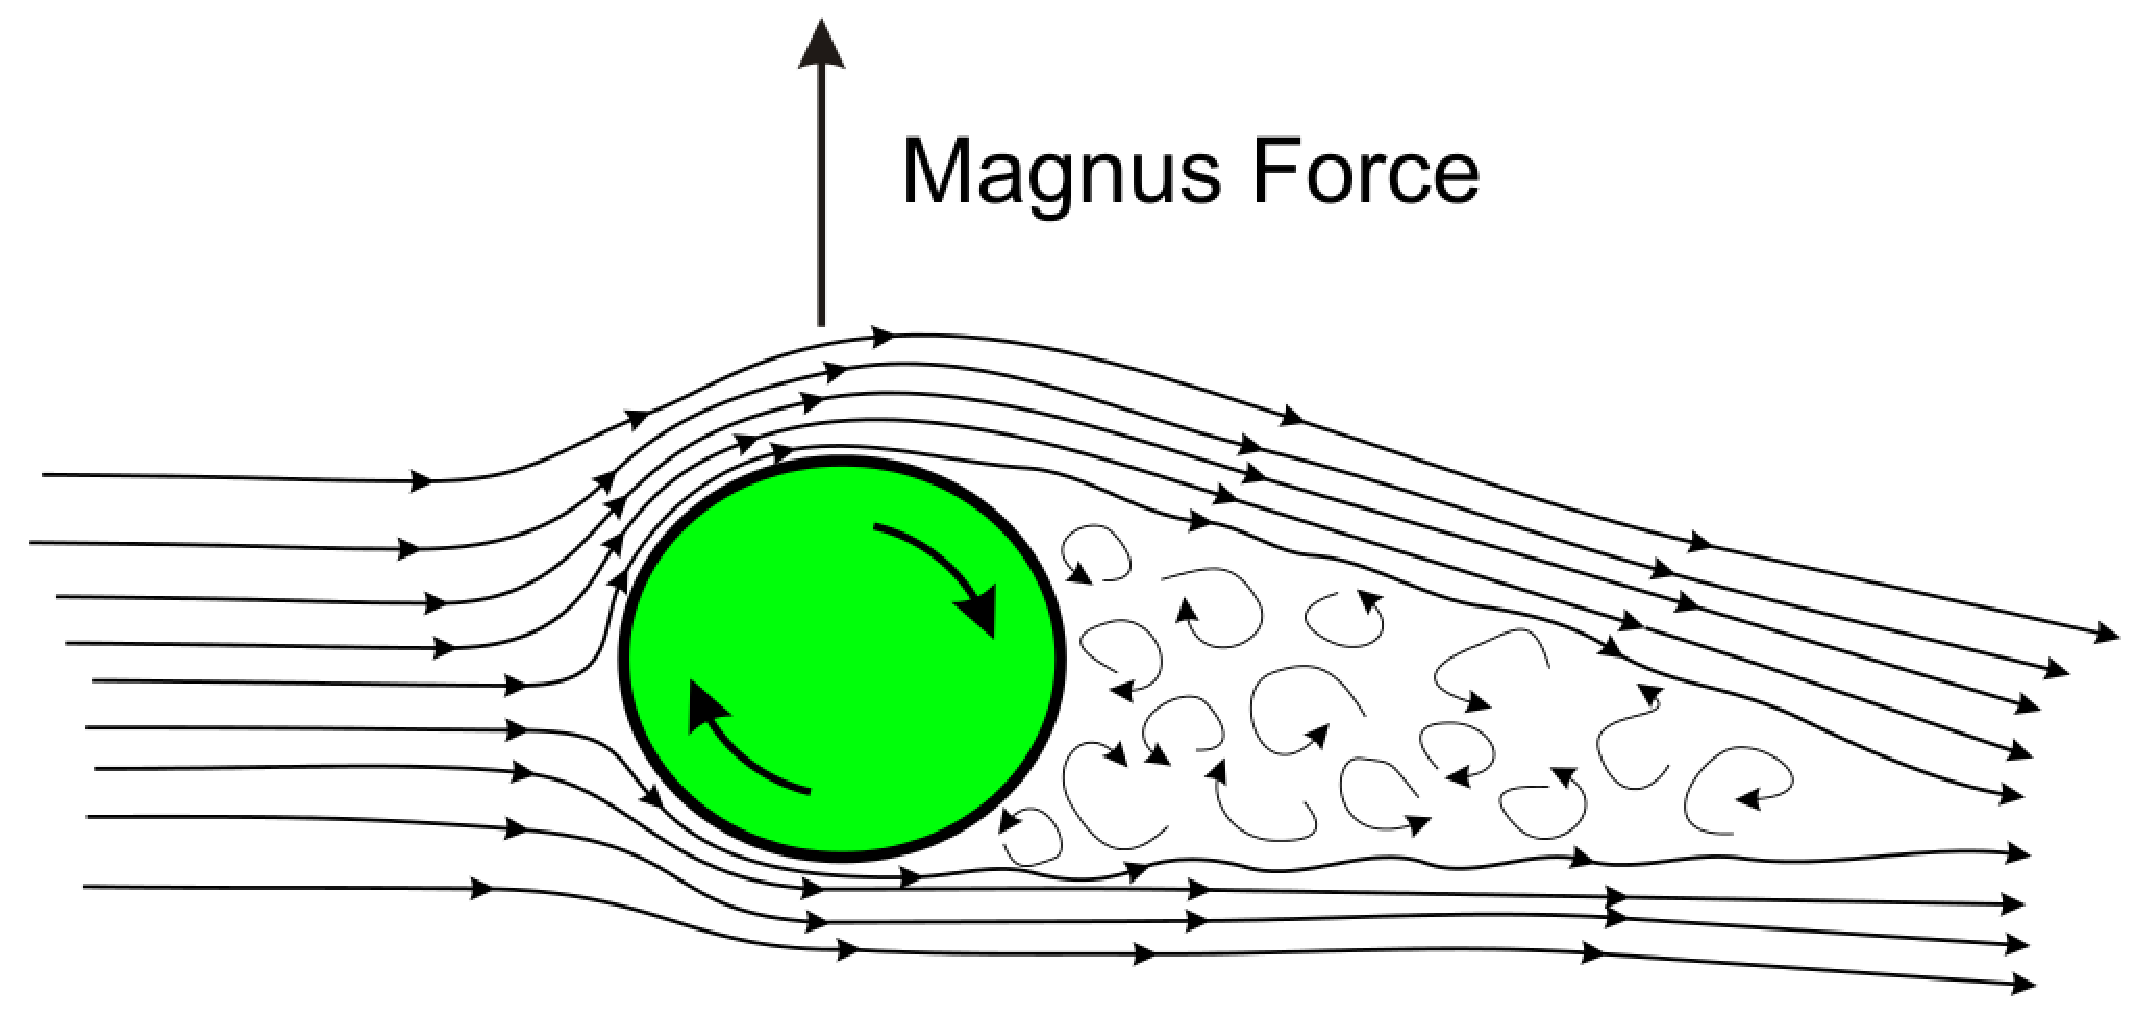
\includegraphics[scale=0.45]{../images/magnus.pdf}
\caption[A diagram of the Magnus effect]{A diagram of the Magnus force on a rotating sphere.
Adapted from \url{http://en.wikipedia.org/wiki/File:Sketch_of_Magnus_effect_with_streamlines_and_turbulent_wake.svg}.}
\label{magnus}
\end{figure}

\subsection{The Drag Crisis} \label{sec:drag-crisis}

When measuring the flow around a smooth sphere, one finds a curious phenomenon. At approximately
$Re = 2\times10^5$ the drag coefficient on the sphere suddenly decreases from around $c_D = 0.4$ 
to $c_D = 0.1$. This sudden change in drag is associated with the boundary layer around the sphere
becoming turbulent and the wake behind the ball, as described before, becoming shorter and thinner as
compared to the size of the ball.

Modelling this transition to turbulence is incredibly difficult, even for smooth spheres, and is 
incredibly difficult for the case of a dimpled golf ball. We must make do with measurements from 
experiments to understand the behaviour of $c_D$ as the Reynolds number varies.

In \citet{Morrison2010} all experimental data for the drag on a smooth sphere is combined to give a
formula for the drag in the Reynolds number range $Re = 1$ to $Re = 10^6$. This combined
form exhibits the drag crisis drop at around $Re = 2\times10^5$ experiments have seen, and is given by
\begin{equation} \label{drag-m}
c_D = \frac{24}{Re} + \frac{2.6(Re/5)}{1 + (Re/5)^{1.52}} + \frac{0.411(Re/263000)^{-7.94}}{1+(Re/263000)^{-8.00}}
+ \frac{Re^{0.8}}{461000} .
\end{equation}
using experimental results found from \citet{schlichting1968boundary}.
\begin{figure}[h]
\centering
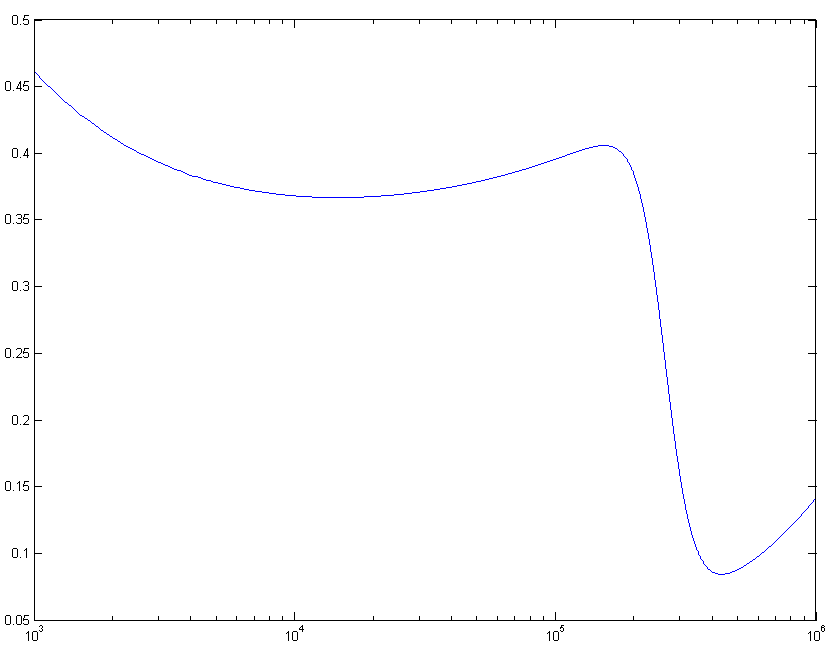
\includegraphics[scale=0.7]{../images/morrison-drag.png}
\caption[Plot of the Morrison drag formula]{A plot of the Morrison drag formula from $Re = 10^3$ to
$Re=10^6$. Note the sudden drop in drag at around $Re = 2\times10^5$ as expected.}
\end{figure}

For a golf ball, the presence of dimples on the surface of the ball serves to reduce the Reynolds
number at which the drag crisis occurs \citet{Bearman1976}, moving the range of speeds where the golf
ball is in the low drag (supercritical) region to within the capability of a human golfer to hit. This
vast reduction in drag makes a large difference to the flight of a ball, and we will need to account
for this affect in any model we form.

The mechanism by which this reduction in drag occurs is the boundary layer around the body becoming 
turbulent. This turbulence delays boundary layer separation (keeping the layer on the body closer to
the back) and thus reduces the size of the wake which results when the boundary layer separates. Reducing
the size of the wake has the effect of reducing the pressure difference between the front of the body
and the back, overall reducing the drag.

The configuration of the dimples on the ball also has a large effect on the values of $Re$ at which 
the drag crisis occurs, and the value of $c_D$ at either side of the drop \citet{Naruo2014}. The dimples
serve to introduce vortices, and thus encourage turbulence, at a lower value of Reynolds number. There is
a large variation between particular type of ball (see Figure 3 in \citet{Naruo2014}), which mean that
individual balls can likely be characterised simply in terms of their drag function.

\section{Previous Work on Modelling Golf Ball Flight}

There has been considerable attention within the literature on the topic of modelling the flight of a
golf ball, both due to the considerable industry surrounding the game and the interesting fluid
dynamics which results from golf ball flight. A small selection of such papers are
\citet{Smits2004,Bearman1976,Penner2003,Alam2011,Kensrud2010,Leong2007} however there are many more
which could be discussed.

The earliest of these papers is \citet{Bearman1976} which is one of the first attempts
to understand the fluid dynamics over a golf ball and provide a model for the flight of a ball taking
this into account. The drag crisis on a golf ball is shown in experimental data taken from an earlier
paper and from measurements the authors made in a wind tunnel. These measurements were taken at a range
of $Re$ values and spin values, providing a useful set data to correlate any findings against. The
paper also emphasizes the importance of the dimples on the aerodynamic characteristics of the ball,
in agreement with other papers.

In \citet{Smits2004} the authors summarise the main effects one will find on golf ball trajectories,
mentioning both the laminar and turbulent boundary layer we discussed previously, the effect of spin
on the lift coefficient, and including some of the data from \citet{Bearman1976} to illustrate these
points. The paper also suggests that much work still remains in understanding how the fluid dynamics
over golf balls functions, saying that fundamentally balls are designed via empirical means, simply
using the knowledge contained in the previous sections and experiments to improve the designs of balls.
The authors state also state, with reference to the design of golf balls \citet[page 10]{Smits2004}:

``The fundamental design challenge in optimizing golf ball aerodynamics is achieving the lower possible drag level at high Reynolds number while ensuring a high lift coefficient at the lowest Reynolds number in the design space.''

These two goals are virtually at opposite ends from each other and thus means the challenge of making
a good golf ball for all ranges of speed in a typical game is very difficult.

There are a number of papers exclusively on experimental measurements of drag and lift on golf balls, 
for example \citet{Bearman1976}, \citet{Kharlamov2007Magnus}, \citet{Naruo2014}, \citet{Kray2012} and \citet{Aoki2010}.
All of these papers show evidence for the drag crisis at lower Reynolds number than a smooth sphere,
and for the Magnus effect on on flight. \citet{Aoki2010} gives a value for the transition to the
supercritical drag regime as $Re = 0.5\times10^5$ which is slightly lower than the values given in
other references. However, this can be accounted for by noting that this measurement is taken without
rotation and potentially with a different ball to other references. Additionally, this paper contains
direct measurements of the boundary layer separation on both sides of a rotating ball, and finds 
excellent agreement between the expected behaviour and the real physical behaviour.

\citet{Kray2012} focuses on the Magnus effect predominantly, and takes experimental measurements on
larger spheres than a golf ball. However, these measurements are in a similar Reynolds number range
to the case for golf and so the results here could be of some use. The authors also report observing
the negative Magnus effect in their tests. However, some of the results within in this report are
obtained using a sphere attached to two rods in a wind tunnel which could significantly affect the fluid flow
in the boundary layer, a point the authors themselves concede.

Finally, in \citet{Naruo2014} the effects of differing the depth of the dimpling on a golf ball is 
explored at a range of flow speeds. The authors find that even small changes to the dimple configuration 
(a change in depth of 0.035mm)
can have large effects on the lift on the ball and thus the resultant trajectory. Additionally, the
authors attempt a strategy with a ball with smaller dimples placed between the normal sized dimples
a standard golf ball. They report a increase in the carry of the ball of approximately 8m. While we will not 
investigate into the dimpling on the ball, it is interesting to see the directions that golf ball
technology may advance in the future.

\subsection{Computational Simulations of Golf Ball Flight}

Performing accurate computational simulations of the flow over a golf ball is a particularly large 
challenge. The complex turbulent wake behind a golf ball, and the potential for the turbulent boundary
layer, along with the rotation and high Reynolds numbers the flow typically operate in mean that any
computational simulations will need both small time stepping and large mesh sizes to deal with the 
resultant flow.

It is only recently that such simulations have become feasible using super computers with large numbers
of cpu cores and memory. Parallelisation of these methods means that systems with large numbers of
cpu cores can dramatically cut down the time that such simulations take.

The first paper to attempt a full simulation of the flow over a non spinning ball for a range of
Reynolds numbers was \citet{Smith2010}. The authors use a fairly sophisticated discretisation method
for the points within the domain, dividing them into interior points within the ball, forcing points
directly on the boundary which have different boundary conditions, and fluid points. Each of these has
different behaviour to the other, and some interpolation methods are used to bridge the gap between
the values at each set of points. This methodology is used as the points do not have to fit around
the boundary of the ball, allowing a much simpler Cartesian grid to be used instead of attempting to
use a grid set in a spherical coordinate system with the ball.

The solution is based on solving the full Navier Stokes equations, \eqref{incompress} and \eqref{momentum}
around the golf ball for the flow, using a Crank-Nicholson method for the viscous terms and using
a third order Runge-Kutta scheme for the other terms. The ball modelled has 300 dimples, a fairly
typical configuration.

The results are in good line with the behaviour we expect to see for Reynolds numbers between the
subcritical (here $Re = 2.5\times10^4$) and supercritical ($Re = 1.1\times10^5$) regimes, finding the 
drag crisis drop that experiments have observed.
The authors also obtain visualisations of the flow over the ball in the two different regimes, finding
the transition to turbulence in the boundary layer in the supercritical range and the turbulent wake 
behind the ball.

\citet{Beratlis2012Numerical} extends this work to spinning golf balls, and samples from a different
set of Reynolds number, this time in the subcritical domain $Re = 1.7\times10^4$, during the critical
Reynolds number drop $Re = 4.5\times10^4$ and $Re = 6.5\times10^4$, and in the supercritical section
at $Re = 1.7\times10^5$. This study uses a more sophisticated grid setup in cylindrical coordinates,
with a similar hybrid explicit and implicit scheme to solve the Navier-Stokes equations around the ball.

The computational resources used within this study are quite considerable: at the lowest Reynolds 
number considered the grid size is approximately $3\times10^7$ points, and the authors estimate that each rotation
takes $1800$ hours of cpu time to compute. By the final and largest Reynolds number considered, and at 
highest spin, the grid is increased by over 5 times to approximately $1.5\times10^8$ points, 
and the authors estimate this
takes $260000$ hours of cpu time to compute.

These investigations find a similar result to both the experiments and the previous work in \citet{Smith2010},
seeing all the features we would expect and following the experimental data quite closely.

Finally, in \citet{Aoki2010} some numerical simulations of the flow using the FLUENT fluid dynamics
software are undertaken. The authors only obtained a few results, and crucially only one result after
the advent of the drag crisis. While the results they find are broadly within line with the expected
experimental results there are too few to really validate the accuracy of the technique.

Using computational fluid modelling over golf balls is still in its infancy, and there is a long way
to go until the technique is sufficiently accurate to be able to easily model different types of ball.
The huge computational resources required are a problem, however as computers grow more powerful and
generally have more cores this will come within the range of researchers to quickly simulate the flow
over a ball.

\section{Measuring Golf Ball Trajectories}

Golf ball trajectories can be measured in a number of ways, depending on the distance over which we
wish to take the measurements. There are setups over small ranges which use cameras to track the ball
during its flight, however these are limited in the range at which the ball can be distinguished by
the camera.

In this project, the data we have been supplied with predominantly uses Doppler radar to measure the
full trajectory of the flight. This allows both the position of the ball over the flight to be found
and the spin, by virtue of the use of the Doppler effect to measure the rotational motion of the ball.

It is possible to also use this Doppler radar technique to estimate the $c_D$ at each point of the 
flight, as is described in \citet{Martin2012} for the case of baseballs.

\section{Summary}

The fluid dynamics occurring during golf ball flight is highly complex, with a number of different affects 
present during the flight. We have considered only the main affects on a spinning sphere which
manifest themselves during golf ball flight. There are other phenomena which could be discussed, 
for example the Basset force \citet{thomas1992influence}, which we have not considered.

Understanding the form which $c_D$ and $c_L$ take for a golf ball is a large part of this project.
From the fluid mechanics we have considered in this chapter we note that we will expect these functions
to depend on the Reynolds number, and for the lift to additionally have some dependency on $\omega$ the
angular velocity of the ball.

Understanding the exact nature of the fluid mechanics on each and every ball is still incredibly
difficult with the turbulent flow over the ball. As such, any parametrisations of the golf ball
characteristics will inevitably be an approximation to the true nature of how this system works.